\documentclass[10pt]{article}
\usepackage{ctex}
\usepackage[top=1.6cm, bottom=1.6cm, left=0.5cm, right=0.5cm]{geometry}
\usepackage{multicol}
\usepackage{amsmath}
\usepackage{amsfonts}
\usepackage{amssymb}
\usepackage{graphicx}

\setlength{\parindent}{0pt}
\setlength{\parskip}{1pt}
\setlength{\columnsep}{12pt}
\setlength{\columnseprule}{0pt}

\begin{document}

\begin{multicols*}{3}
\raggedcolumns

\section*{导数公式}
\vspace{-8pt}

\[\frac{d}{dx}\tan x = \sec^2 x\]
\[\frac{d}{dx}\sec x = \tan x \sec x\]
\[\frac{d}{dx}\cot x = -\csc^2 x\]
\[\frac{d}{dx}\csc x = -\csc x \cot x\]
\[\frac{d}{dx}a^x = a^x \ln a\]
\[\frac{d}{dx}\log_a x = \frac{1}{x \ln a}\]
\[\frac{d}{dx}\arcsin x = \frac{1}{\sqrt{1 - x^2}}\]
\[\frac{d}{dx}\arccos x = -\frac{1}{\sqrt{1 - x^2}}\]
\[\frac{d}{dx}\arctan x = \frac{1}{1 + x^2}\]
\[\frac{d}{dx}\cot^{-1} x = -\frac{1}{1 + x^2}\]
\[\frac{d}{dx}[\ln(x + \sqrt{1 + x^2})] = \frac{1}{\sqrt{1 + x^2}}\]

\section*{三角函数}
\vspace{-8pt}

\[\sec x = \frac{1}{\cos x}, \quad \csc x = \frac{1}{\sin x}, \quad \cot x = \frac{\cos x}{\sin x}\]
% cos和tan的关系 平方倒数加一
\[\sec^2 x = 1 + \tan^2 x, \quad \csc^2 x = 1 + \cot^2 x\]
% sec方减tan方 = 1
\[\sec^2 x - \tan^2 x = 1, \quad \csc^2 x - \cot^2 x = 1\]

\columnbreak  % 强制换列

\section*{积分公式}
\vspace{-8pt}

\[\int \sec^2 x \, dx = \tan x + C\]
\[\int \tan x \sec x \, dx = \sec x + C\]
\[\int \csc^2 x \, dx = -\cot x + C\]
\[\int \csc x \cot x \, dx = -\csc x + C\]
\[\int a^x \, dx = \frac{a^x}{\ln a} + C\]
\[\int \frac{1}{\sqrt{1 - x^2}} \, dx = \arcsin x + C\]
\[\int \frac{1}{1 + x^2} \, dx = \arctan x + C\]
\[\int \frac{1}{a^2 + x^2} \, dx = \frac{1}{a} \arctan \frac{x}{a} + C\]
\[\int \frac{1}{\sqrt{a^2 - x^2}} \, dx = \arcsin \frac{x}{a} + C\]
\[\int \frac{1}{x \sqrt{x^2 - a^2}} \, dx = \frac{1}{a} \text{arcsec} \frac{x}{a} + C\]
\[\int \frac{1}{x \sqrt{1 + x^2}} \, dx = -\frac{1}{\sqrt{1 + x^2}} + C\]
\[\int \frac{1}{1 + e^x} \, dx = x - \ln(1 + e^x) + C\]
\[\int \ln x \, dx = x \ln x - x + C\]
\[\int \sec x \, dx = \ln|\sec x + \tan x| + C\]
\[\int \csc x \, dx = -\ln|\csc x + \cot x| + C\]
\[\int x^n \, dx = \frac{x^{n+1}}{n+1} + C \quad (n \neq -1)\]
\[\int \frac{1}{1 + e^{-x}} \, dx = \ln(1 + e^x) + C\]
\[\int \frac{1}{a^2 - x^2} \, dx = \frac{1}{2a} \ln\left|\frac{a + x}{a - x}\right| + C\]
\[\int \frac{1}{x^2 - a^2} \, dx = \frac{1}{2a} \ln\left|\frac{x - a}{x + a}\right| + C\]

\section*{泰勒公式与等价代换}
\vspace{-8pt}

\textbf{基本等价代换(x→0):}
\[x \sim \sin x \sim \tan x \sim \arcsin x \sim \arctan x\]
\[\ln(1+x) \sim e^x - 1 \sim x\]
\[(1+x)^\alpha - 1 \sim \alpha x \quad (\alpha \neq 0)\]
\[\ln(\cos x) \sim -\frac{x^2}{2}\]
\[1 - \cos x \sim \frac{x^2}{2}\]
\[x - \sin x \sim \frac{x^3}{6}\]
\[\tan x - x \sim \frac{x^3}{3}\]
\[x - \arcsin x \sim -\frac{x^3}{6}\]
\[x - \arctan x \sim \frac{x^3}{3}\]

\textbf{泰勒展开:}
\[e^x = 1 + x + \frac{x^2}{2!} + \frac{x^3}{3!} + \cdots\]
\[\sin x = x - \frac{x^3}{6} + \frac{x^5}{120} + \cdots\]
\[\cos x = 1 - \frac{x^2}{2} + \frac{x^4}{24} + \cdots\]
\[\ln(1+x) = x - \frac{x^2}{2} + \frac{x^3}{3} + \cdots\]
\[(1+x)^\alpha = 1 + \alpha x + \frac{\alpha(\alpha-1)}{2}x^2 + \cdots\]
% arcsinx & arctanx
\[\arcsin x = x + \frac{x^3}{6} + \frac{3x^5}{40} + \cdots\]
\[\arctan x = x - \frac{x^3}{3} + \frac{x^5}{5} - \cdots\]


\textbf{重要极限:}
\[\lim_{x \to 0} \frac{\sin x}{x} = 1\]
\[\lim_{x \to 0} (1+x)^{1/x} = e\]
\[\lim_{x \to 0} [1 + f(x)]^{g(x)} = e^{\lim_{x \to 0} g(x)f(x)}\]

\end{multicols*}

\newpage
\begin{multicols*}{2}
\raggedcolumns


\section*{常用基本极限}
\vspace{-8pt}

\[\lim_{x \to 0} \frac{\sin x}{x} = 1\]
\[\lim_{x \to 0} (1 + \frac{1}{x})^x = e\]
\[\lim_{x \to 0} (1 + x)^{\frac{1}{x}} = e\]
\[\lim_{x \to 0} \frac{a^x - 1}{x} = \ln a \quad (a > 0)\]
\[\lim_{n \to \infty} \sqrt[n]{n} = 1\]
\[\lim_{n \to \infty} \frac{n}{(n + 1)^n} = \frac{1}{e}\]
\[\lim_{x \to \infty} x^{\frac{1}{x}} = 1\]
\[\lim_{n \to \infty} x^n = \begin{cases} 0, & |x| < 1 \\ \infty, & |x| > 1 \\ 1, & x = 1 \\ 0, & x = -1 \end{cases}\]
\[\lim_{n \to \infty} e^{nx} = \begin{cases} 0, & x < 0 \\ \infty, & x > 0 \\ 1, & x = 0 \end{cases}\]
\[\lim_{n \to \infty} \frac{a_n + 1}{a_n} = A, \text{若} |A| < 1, \text{则} \lim_{n \to \infty} a_n = 0\]
\[\lim_{x \to \infty} x^\alpha \ln x = 0 \quad (\alpha > 0)\]
\[\lim_{n \to \infty} \sqrt[n]{a_1^n + a_2^n + \cdots + a_k^n} = \max\{a_1, a_2, \ldots, a_k\}\]

\section*{间断点分类}
\vspace{-8pt}

\textbf{第一类间断点:} \(\lim_{x \to x_0^-} f(x) = \lim_{x \to x_0^+} f(x)\) 存在(但不等于 \(f(x_0)\))。

\textbf{可去间断点:} \(\lim_{x \to x_0} f(x)\) 存在,但 \(f(x_0)\) 不存在或不等于 \(\lim_{x \to x_0} f(x)\)。

\textbf{跳跃间断点:} \(\lim_{x \to x_0^-} f(x) \neq \lim_{x \to x_0^+} f(x)\)。

\textbf{第二类间断点:} \(\lim_{x \to x_0^-} f(x)\) 和 \(\lim_{x \to x_0^+} f(x)\) 至少有一个不存在。

\textbf{无穷间断点:} \(\lim_{x \to x_0^-} f(x) = \pm \infty\) 或 \(\lim_{x \to x_0^+} f(x) = \pm \infty\)。

\textbf{振荡型间断点:} \(\lim_{x \to x_0} f(x)\) 不存在,但 \(f(x)\) 在 \(x_0\) 附近振荡。


\section*{极值、最值、拐点}
\vspace{-8pt}
\textbf{极值可能条件:}
\begin{itemize}
  \item \(f'(x_0) = 0\)(驻点)
  \item \(f'(x_0)\) 不存在
\end{itemize}

\textbf{二阶导数判别法:}
\begin{itemize}
  \item 若 \(f''(x_0) > 0\),极小值(凹)
  \item 若 \(f''(x_0) < 0\),极大值(凸)
\end{itemize}

\textbf{高阶导数判别法:}
\begin{itemize}
  \item 若 \(f'(x_0) = f''(x_0) = \cdots = f^{(n-1)}(x_0) = 0\) 且 \(f^{(n)}(x_0) \neq 0\)
  \item \(n\) 为偶数:
    \begin{itemize}
      \item \(f^{(n)}(x_0) > 0\):极小值
      \item \(f^{(n)}(x_0) < 0\):极大值
    \end{itemize}
  \item \(n\) 为奇数:无极值
\end{itemize}

\textbf{拐点判别法:}
\begin{itemize}
  \item \(f''(x_0) = 0\) 或 \(f''(x_0)\) 不存在
  \item \(f''(x)\) 在 \(x_0\) 两侧变号
  \item 若 \(y = f(x)\) 在 \(x_0\) 处三阶可导且 \(f'''(x_0) \neq 0\),则 \((x_0, f(x_0))\) 是拐点
\end{itemize}

\section*{渐近线与曲率}
\vspace{-8pt}

\textbf{渐近线:}
\begin{itemize}
  \item 水平渐近线:若 \(\lim_{x \to \infty} f(x) = A\),则 \(y = A\)
  \item 垂直渐近线:若 \(\lim_{x \to x_0} f(x) = \infty\),则 \(x = x_0\)
  \item 斜渐近线:
    \begin{itemize}
      \item 若 \(\lim_{x \to \infty} \frac{f(x)}{x} = a\) 且 \(\lim_{x \to \infty} [f(x) - ax] = b\),则 \(y = ax + b\)
      \item 若 \(f(x) = ax + b + o(1)\) 且 \(a \neq 0\),则 \(y = ax + b\) 是斜渐近线
    \end{itemize}
\end{itemize}

\textbf{曲率:}
\begin{itemize}
  \item 直角坐标:\(k = \frac{|y''|}{(1 + (y')^2)^{3/2}}\)
  \item 参数方程:\(k = \frac{|x'y'' - y'x''|}{(x'^2 + y'^2)^{3/2}}\)
  \item 曲率半径:\(R = \frac{1}{k}\)
  \item 曲率中心:\((x_0, y_0)\) 处的曲率中心为 \((x_0 - \frac{y'^3 + y'}{y''} , y_0 + \frac{y'^2 + 1}{y''})\)
\end{itemize}

\end{multicols*}

\newpage
\begin{multicols*}{2}
\raggedcolumns

\section*{常用定理}

\textbf{1. 介值定理:}
\begin{itemize}
  \item \(f(x)\) 在 \([a, b]\) 连续,\(f(a) \neq f(b)\),\(C \in (f(a), f(b))\)
  \item 则 \(\exists \xi \in (a, b)\),使得 \(f(\xi) = C\)
\end{itemize}

\textbf{2. 积分中值定理:}
\begin{itemize}
  \item \(f(x)\) 在 \([a, b]\) 连续
  \item 则 \(\exists \xi \in (a, b)\),使得 \(\int_a^b f(x) \, dx = f(\xi)(b - a)\)
\end{itemize}

\textbf{3. 广义积分中值定理:}
\begin{itemize}
  \item \(f(x), g(x)\) 在 \([a, b]\) 上连续,且 \(g(x)\) 不变号
  \item 则 \(\exists \xi \in (a, b)\),使得 \(\int_a^b f(x)g(x) \, dx = f(\xi) \int_a^b g(x) \, dx\)
\end{itemize}

\textbf{4. 零点定理:}
\begin{itemize}
  \item \(f(x)\) 在 \([a, b]\) 连续,且 \(f(a) \cdot f(b) < 0\)
  \item 则 \(\exists \xi \in (a, b)\),使得 \(f(\xi) = 0\)
\end{itemize}

\textbf{5. 罗尔定理:}
\begin{itemize}
  \item \(f(x)\) 在 \([a, b]\) 连续,\((a, b)\) 可导,且 \(f(a) = f(b)\)
  \item 则 \(\exists \xi \in (a, b)\),使得 \(f'(\xi) = 0\)
\end{itemize}

\textbf{6. 拉格朗日中值定理:}
\begin{itemize}
  \item \(f(x)\) 在 \([a, b]\) 连续,\((a, b)\) 可导
  \item 则 \(\exists \xi \in (a, b)\),使得 \(f(b) - f(a) = f'(\xi)(b - a)\) 或 \(\frac{f(b) - f(a)}{b - a} = f'(\xi)\)
\end{itemize}

\textbf{7. 柯西中值定理:}
\begin{itemize}
  \item \(f(x), g(x)\) 在 \([a, b]\) 连续,\((a, b)\) 可导,且 \(g'(x) \neq 0\)
  \item 则 \(\exists \xi \in (a, b)\),使得 \(\frac{f(b) - f(a)}{g(b) - g(a)} = \frac{f'(\xi)}{g'(\xi)}\)
\end{itemize}

\textbf{8. 皮亚诺型余项泰勒公式:}
\begin{itemize}
  \item \(f(x) = f(x_0) + f'(x_0)(x - x_0) + \frac{1}{2!}f''(x_0)(x - x_0)^2 + \cdots + \frac{1}{n!}f^{(n)}(x_0)(x - x_0)^n + o[(x - x_0)^n]\)
\end{itemize}

\textbf{9. 拉格朗日型余项泰勒公式:}
\begin{itemize}
  \item \(f(x) = f(x_0) + f'(x_0)(x - x_0) + \frac{1}{2!}f''(x_0)(x - x_0)^2 + \cdots + \frac{1}{n!}f^{(n)}(x_0)(x - x_0)^n + R_n(x)\)
  \item \(R_n(x) = \frac{f^{(n+1)}(\xi)}{(n+1)!}(x - x_0)^{n+1}\) 其中 \(\xi\) 在 \(x_0\) 与 \(x\) 之间
\end{itemize}

\textbf{10. 一阶线性微分方程 \(y' + p(x)y = q(x)\):}
\begin{itemize}
  \item 通解公式:\(y = e^{-\int p(x)dx} \left[ \int q(x) e^{\int p(x)dx} dx + C \right]\)
\end{itemize}

\textbf{11. 齐次通解 + 非齐次特解 = 非齐次通解:}
\begin{itemize}
  \item 两个非齐次方程特解的差是齐次方程的解
\end{itemize}

\section*{定积分性质}
\vspace{-8pt}

\textbf{奇偶性:}
\[\int_{-a}^a f(x)dx = \begin{cases} 
0, & f(x) \text{为奇函数} \\
2\int_0^a f(x)dx, & f(x) \text{为偶函数}
\end{cases}\]

\textbf{周期性:}
\[\int_a^{a+T} f(x)dx = \int_0^T f(x)dx\]

\textbf{华莱士(点火)公式:}
\begin{itemize}
  \item \(\int_0^{\frac{\pi}{2}} \sin^n x dx = \int_0^{\frac{\pi}{2}} \cos^n x dx = \begin{cases} 
  \frac{n-1}{n} \cdot \frac{n-3}{n-2} \cdots \frac{1}{2} \cdot \frac{\pi}{2}, & n \text{为偶数} \\
  \frac{n-1}{n} \cdot \frac{n-3}{n-2} \cdots \frac{2}{3}, & n \text{为奇数}
  \end{cases}\)
  \item \(\int_0^{2\pi} \sin^n x dx = \int_0^{2\pi} \cos^n x dx = \begin{cases} 
  4\int_0^{\frac{\pi}{2}} \sin^n x dx, & n \text{为偶数} \\
  0, & n \text{为奇数}
  \end{cases}\)
  \item \(\int_0^{\frac{\pi}{2}} x f(\sin x)dx = \frac{\pi}{2}\int_0^{\frac{\pi}{2}} f(\sin x)dx\)
  \item \(\int_0^{\pi} x \sin x dx = \frac{\pi}{2}\int_0^{\pi} \sin x dx = \pi\)
\end{itemize}

\textbf{定积分几何意义:}
\begin{itemize}
  \item \(\int_0^a \sqrt{a^2 - x^2}dx = \frac{\pi a^2}{4}\)
  \item \(\int_a^{2a} \sqrt{2ax - x^2}dx = \frac{\pi a^2}{4}\)
  \item \(\int_0^{2a} \sqrt{2ax - x^2}dx = \frac{\pi a^2}{2}\)
\end{itemize}

\section*{定积分可积性}
\vspace{-8pt}

\begin{itemize}
  \item \textbf{必要条件:} 若 \(\int_a^b f(x)dx\) 存在,则 \(f(x)\) 在 \([a,b]\) 上有界
  \item \textbf{充分条件:} \(f(x)\) 在 \([a,b]\) 上连续,则 \(\int_a^b f(x)dx\) 存在
  \item \(f(x)\) 在 \([a,b]\) 上有界,且只有有限个间断点,则 \(\int_a^b f(x)dx\) 存在
  \item \(f(x)\) 在 \([a,b]\) 上只有有限个第一类间断点,则 \(\int_a^b f(x)dx\) 存在
\end{itemize}

\section*{变上限积分求导性质}
\vspace{-8pt}

\begin{itemize}
  \item \(F(x) = \int_a^x f(t)dt\)
  \item \textbf{连续性:} \(f(x)\) 在 \([a,b]\) 上可积,则 \(F(x)\) 在 \([a,b]\) 上连续
  \item \textbf{可导性:}
    \begin{itemize}
      \item \(f(x)\) 连续,则 \(F'(x) = f(x)\)
      \item \(f(x)\) 可去间断,则 \(F'(x) = \lim_{t \to x} f(t)\)
    \end{itemize}
  \item \(f(x)\) 连续但不可导,且 \(F(x)\) 在 \(x_0\) 处连续,\(F'_-(x_0) = f(x_0^-)\),\(F'_+(x_0) = f(x_0^+)\)
\end{itemize}


\end{multicols*}

\newpage
\begin{multicols*}{2}
\raggedcolumns


\section*{收敛性}
\vspace{-8pt}

\textbf{基本定理:}
\begin{itemize}
  \item \(f(x), g(x)\) 在 \([a,+\infty)\) 上连续,且 \(0 \leq f(x) \leq g(x)\)
  \item \(\int_a^{+\infty} g(x)dx\) 收敛 \(\Rightarrow\) \(\int_a^{+\infty} f(x)dx\) 收敛
  \item \(\int_a^{+\infty} f(x)dx\) 发散 \(\Rightarrow\) \(\int_a^{+\infty} g(x)dx\) 发散
\end{itemize}

\textbf{极限比较判别法:}
\begin{itemize}
  \item \(\lim_{x \to +\infty} \frac{f(x)}{g(x)} = C\)(有限或无穷)
  \item \(C > 0\): \(\int_a^{+\infty} f(x)dx, \int_a^{+\infty} g(x)dx\) 同敛散
  \item \(C = 0\): 若 \(\int_a^{+\infty} g(x)dx\) 收敛,则 \(\int_a^{+\infty} f(x)dx\) 收敛
  \item \(C = +\infty\): 若 \(\int_a^{+\infty} g(x)dx\) 发散,则 \(\int_a^{+\infty} f(x)dx\) 发散
\end{itemize}

\textbf{常见 \(P\) 积分:}
\begin{itemize}
  \item \(\int_a^{+\infty} \frac{1}{x^p}dx\):\(p > 1\) 收敛,\(p \leq 1\) 发散
  \item \(\int_a^b \frac{1}{(x - a)^p}dx\):\(p < 1\) 收敛,\(p \geq 1\) 发散
  \item \(\int_a^b \frac{1}{(b - x)^p}dx\):同上
\end{itemize}

\section*{多元极值与最值}
\vspace{-8pt}

\textbf{极值:}
\begin{itemize}
  \item \textbf{方法:}
    \begin{itemize}
      \item 求偏导 \(Z_x, Z_y\),令 \(Z_x = 0, Z_y = 0\) 找驻点
      \item 求 \(A = Z_{xx}, B = Z_{xy}, C = Z_{yy}\),代入驻点判断 \(AC - B^2\)
    \end{itemize}
  \item \textbf{判断:}
    \begin{itemize}
      \item \(AC - B^2 > 0\): 极值点
        \begin{itemize}
          \item \(A < 0\):极大值点
          \item \(A > 0\):极小值点
        \end{itemize}
      \item \(AC - B^2 < 0\):不是极值点
      \item \(AC - B^2 = 0\):不确定,用定义判定
    \end{itemize}
\end{itemize}

\textbf{最值:}
\begin{itemize}
  \item 求 \(f(x,y)\) 在区域内部可能极值点
  \item 求 \(f(x,y)\) 在边界上的最大最小值
  \item 比较所有候选值得到最值
\end{itemize}


\section*{多元微分}

\textbf{连续性:} 若 \(\lim_{(x,y) \to (x_0,y_0)} f(x,y) = f(x_0,y_0)\),则称 \(f(x,y)\) 在点 \((x_0,y_0)\) 连续。

\textbf{偏导数:}
\[
f_x(x_0,y_0) = \lim_{\Delta x \to 0} \frac{f(x_0 + \Delta x,y_0) - f(x_0,y_0)}{\Delta x} = \frac{d}{dx} f(x,y_0)\bigg|_{x=x_0}
\]
\[
f_y(x_0,y_0) = \lim_{\Delta y \to 0} \frac{f(x_0,y_0 + \Delta y) - f(x_0,y_0)}{\Delta y} = \frac{d}{dy} f(x_0,y)\bigg|_{y=y_0}
\]

\textbf{可微性:} \(f(x,y)\) 在点 \((x_0,y_0)\) 处可微的等价形式:
\begin{itemize}
  \item \(\Delta z = f(x_0 + \Delta x,y_0 + \Delta y) - f(x_0,y_0) = A \Delta x + B \Delta y + o(\rho)\),其中 \(f_x(x_0,y_0) = A\),\(f_y(x_0,y_0) = B\)
  \item \(\lim_{\rho \to 0} \frac{f(x_0 + \Delta x,y_0 + \Delta y) - f(x_0,y_0) - (A \Delta x + B \Delta y)}{\rho} = 0\)
  \item \(\Delta z = f(x,y) - f(x_0,y_0) = A(x - x_0) + B(y - y_0) + o(\rho)\)
  \item \(\lim_{(x,y) \to (x_0,y_0)} \frac{f(x,y) - f(x_0,y_0) - [A(x - x_0) + B(y - y_0)]}{\sqrt{(x - x_0)^2 + (y - y_0)^2}} = 0\)
\end{itemize}

\textbf{可微性的判断:}
\begin{itemize}
  \item \textbf{必要条件:} \(f_x(x_0,y_0)\) 和 \(f_y(x_0,y_0)\) 都存在
  \item \textbf{充分条件:} \(f_x(x,y)\) 和 \(f_y(x,y)\) 在 \((x_0,y_0)\) 连续
  \item \textbf{用定义判断:}
    \begin{itemize}
      \item \(f_x(x_0,y_0)\) 和 \(f_y(x_0,y_0)\) 是否都存在?
      \item \(\lim_{\substack{\Delta x \to 0 \\ \Delta y \to 0}} \frac{f(x_0 + \Delta x,y_0 + \Delta y) - f(x_0,y_0) - [f_x(x_0,y_0)\Delta x + f_y(x_0,y_0)\Delta y]}{\sqrt{(\Delta x)^2 + (\Delta y)^2}}\) 是否为零?
    \end{itemize}
\end{itemize}

\section*{隐函数求导法则}

\(F(x,y,z) = 0\) 确定 \(z = z(x,y)\):
\begin{itemize}
  \item \(\frac{\partial z}{\partial x} = -\frac{F_x}{F_z}\),\(\frac{\partial z}{\partial y} = -\frac{F_y}{F_z}\)
  \item 对等式两边直接对 \(x\) 或 \(y\) 求导
  \item 微分形式不变性:\(F_x dx + F_y dy + F_z dz = 0\)
\end{itemize}

\end{multicols*}

\newpage
\begin{multicols}{2}
\raggedcolumns


\section*{二重积分}

\textbf{极坐标变换:}
\begin{itemize}
  \item \(d\sigma = d\theta \cdot r dr\)
  \item \(\sin\theta + \cos\theta = \sqrt{2}\sin(\theta + \frac{\pi}{4})\)
  \item \(\sin\theta - \cos\theta = \sqrt{2}\sin(\theta - \frac{\pi}{4})\)
\end{itemize}

\textbf{对称性:}
\begin{itemize}
  \item 积分域 \(D\) 关于 \(y\) 轴对称,\(f(x,y)\) 关于 \(x\) 有奇偶性:
    \begin{itemize}
      \item \(\iint_D f(x,y) d\sigma = \begin{cases} 2\iint_{D_{x>0}} f(x,y) d\sigma, & f(x,y) \text{关于 } x \text{ 为偶函数} \\ 0, & f(x,y) \text{关于 } x \text{ 为奇函数} \end{cases}\)
    \end{itemize}
  \item 积分域 \(D\) 关于 \(x\) 轴对称,\(f(x,y)\) 关于 \(y\) 有奇偶性:
    \begin{itemize}
      \item \(\iint_D f(x,y) d\sigma = \begin{cases} 2\iint_{D_{y>0}} f(x,y) d\sigma, & f(x,y) \text{关于 } y \text{ 为偶函数} \\ 0, & f(x,y) \text{关于 } y \text{ 为奇函数} \end{cases}\)
    \end{itemize}
  \item 积分域 \(D\) 关于 \(y = x\) 对称:
    \begin{itemize}
      \item \(\iint_D f(x,y) d\sigma = \iint_D f(y,x) d\sigma\)
      \item \(\iint_D [f(x,y) + f(y,x)] d\sigma = 2\iint_D f(x,y) d\sigma\)
    \end{itemize}
\end{itemize}

\textbf{应用:}
\begin{itemize}
  \item 平面区域的面积: \(S = \iint_D d\sigma\)
  \item 旋转体的体积:
    \begin{itemize}
      \item 绕 \(x\) 轴旋转: \(V = \pi \int_a^b [f(x)]^2 dx\)
      \item 绕 \(y\) 轴旋转: \(V = \pi \int_c^d [g(y)]^2 dy\)
      \item 绕直线 \(L: ax + by + c = 0\) 旋转: \(r(x,y) = \frac{|ax + by + c|}{\sqrt{a^2 + b^2}}\)
    \end{itemize}
\end{itemize}

\textbf{圆的一般方程:}
\begin{itemize}
  \item \(x^2 + y^2 + Dx + Ey + F = 0\)
  \item 圆心: \(\left(-\frac{D}{2}, -\frac{E}{2}\right)\),半径: \(\frac{\sqrt{D^2 + E^2 - 4F}}{2}\)
\end{itemize}

\end{multicols}

\newpage
\begin{multicols}{2}
\raggedcolumns


\section*{线性代数}

\textbf{行列式:}
\begin{itemize}
  \item 行列式性质
    \begin{itemize}
      \item 转置行列式值不变: \(|A| = |A^T|\)
      \item 行列互换位置,行列式值变号(行列相同,行列式的值变号)
      \item 行列可以提出k,提到行列式外面
      \item 行列可以拆加法
      \item 行列k倍可以加到另一行列上,行列式的值不变
    \end{itemize}
  \item 代数余子式
    \begin{itemize}
      \item 除去第i行第j列的元素,剩下的行列式称为第i行第j列的代数余子式
      \item n阶行列式等于它任意一行列元素与其所对应的代数余子式乘积之和
      \item 行列式的任一行列元素与另一行列元素的代数余子式的乘积之和等于0
      \item 上下三角行列式的值等于主对角线元素的乘积
      \item 副对角线上下三角行列式的值等于
      
      \((-1)^{n(n-1)/2} a_{1n} a_{2(n-1)} \cdots a_{n1}\)
      \item 特殊的拉普拉斯展开公式
        \begin{itemize}
            \item 两个特殊的拉普拉斯展开公式:
            \begin{itemize}
              \item 若 $A$ 和 $B$ 分别是 $m$ 阶和 $n$ 阶方阵,则
              \[
                \left| \begin{matrix} A & * \\ O & B \end{matrix} \right| = |A| \cdot |B|
              \]
              \[
                \left| \begin{matrix} O & A \\ B & * \end{matrix} \right| = \left| \begin{matrix} * & A \\ B & 0 \end{matrix} \right| = (-1)^{m n} |A| \cdot |B|
              \]
                \item 范德蒙德行列式(Vandermonde determinant):
                \[
                V(x_1, x_2, \ldots, x_n) =
                \begin{vmatrix}
                  1 & 1 & \cdots & 1 \\
                  x_1 & x_2 & \cdots & x_n \\
                  x_1^2 & x_2^2 & \cdots & x_n^2 \\
                  \vdots & \vdots & & \vdots \\
                  x_1^{n-1} & x_2^{n-1} & \cdots & x_n^{n-1}
                \end{vmatrix}
                \]
                \[
                \qquad = \prod_{1 \leq i < j \leq n} (x_j - x_i)
                \]       \end{itemize}

        \end{itemize}

      \item 计算行列式的值:朝着单行列只有一个非零元素的方向展开
      \item 克拉默行列式(Cramer's rule):
        \begin{itemize}
          \item 对于线性方程组 \(Ax = b\),其中 \(A\) 是 \(n \times n\) 的矩阵,\(b\) 是 \(n\) 维向量,\(x\) 是未知向量。
          \item 若 \(|A| \neq 0\),则解为:
          \[
          x_i = \frac{|A_i|}{|A|}
          \]
          其中 \(A_i\) 是将矩阵 \(A\) 的第 \(i\) 列替换为向量 \(b\) 后得到的矩阵。
          \item 对于相同的齐次线性方程组 \(Ax = 0\),若 \(|A| \neq 0\),则唯一解为 \(x = 0\)。
          \item 反之,若 \(|A| = 0\),则方程组有无穷多解或无解。
        \end{itemize}
    \end{itemize}

\end{itemize}

\textbf{矩阵}
\begin{itemize}
  \item 注意转置提k:
    \[
    (kA)^T = kA^T
    \]
  \item 方阵的行列式:
    \begin{itemize}
      \item \( |A^T| = |A| \)(转置矩阵的行列式等于原矩阵的行列式)
      \item \( |kA| = k^n |A| \)(\(A\) 为 \(n\) 阶矩阵,\(k\) 为常数)
      \item \( |AB| = |A| |B| \)(矩阵的行列式的乘积等于两个矩阵行列式的乘积)
      \item \( |A^{-1}| = \frac{1}{|A|} \)(可逆矩阵的行列式等于其逆矩阵的行列式的倒数)
      \item A为m阶,B为n阶\\
      \(
        \left| \begin{matrix} A & O \\ C & B \end{matrix} \right| = \left| \begin{matrix} A & D \\ O & B \end{matrix} \right| = |A| \cdot |B|
      \)

      \(
        \left| \begin{matrix} O & A \\ B & C \end{matrix} \right| = \left| \begin{matrix} D & A \\ B & O \end{matrix} \right| = (-1)^{mn} |A| \cdot |B|
      \)
      
    \end{itemize}
  \item 矩阵的逆:
    \begin{itemize}
      \item 伴随矩阵: 每个位置对应的代数余子式的转置矩阵,计作 \(A^*\)
      \item 伴随矩阵的公式:
        \begin{itemize}
          \item \( A A^* = A^* A = |A| E \)
          \item \( (A^*)^{-1} = \frac{1}{|A|} A^* = \frac{1}{|A|} A \)
          \item \( ( k A )^* = k^{n-1} A^* \)(\(A\) 为 \(n\) 阶矩阵)
          \item \( (A^*) = |A| A^{-1} \)(\(A\) 为可逆矩阵)
          \item \( (A^*)^T = (A^T)^* \)(伴随矩阵的转置等于原矩阵的伴随矩阵)
          \item \( |A^*| = |A|^{n-1} \)(\(A\) 为 \(n\) 阶矩阵)
          \item \( (A^*)^* = |A|^{n-2} A \)(\(A\) 为可逆矩阵)
        \end{itemize}
    \end{itemize}
  \item n阶矩阵A可逆的充要条件:
    \begin{itemize}
      \item 存在逆矩阵: \(A^{-1}\) 存在且唯一,\(AB = E\)
      \item 行列式不为零: \(|A| \neq 0\) 或秩 \(r(A) = n\) 
      \item 行列线性无关: \(A\) 的行或列向量线性无关
      \item 齐次线性方程组 \(Ax = 0\) 只有零解
      \item 任意非零向量 \(b\) 的线性方程组 \(Ax = b\) 有唯一解
      \item 矩阵A的特征值全不为0
    \end{itemize}
  \item 逆矩阵的运算性质:
    \begin{itemize}
      \item \((kA)^{-1} = \frac{1}{k} A^{-1}\)(\(k \neq 0\))
      \item \((AB)^{-1} = B^{-1} A^{-1}\),特别地,\((A^2)^{-1} = (A^{-1})^2\)
      \item \((A^{-1})^{-1} = A\), \((A^T)^{-1} = (A^{-1})^T\), \(|A^{-1}| = \frac{1}{|A|}\)
      \item Notice: \((A + B)^{-1} \neq A^{-1} + B^{-1}\)
    \end{itemize}
\end{itemize}

\textbf{矩阵的秩:}
\begin{itemize}
  \item 矩阵的秩:
    \begin{itemize}
      \item 矩阵的秩是矩阵中最大线性无关行或列的个数
      \item 矩阵的秩等于其行列式不为零的最大阶数
      \item 矩阵的秩等于其转置矩阵的秩
      \item 矩阵的秩等于其伴随矩阵的秩
      \item 矩阵的秩等于其行或列向量的线性无关个数即秩
      \item \( r(A) = r \) 矩阵A中非零子式的最大阶数为 \(r\)
      \item \( r(A) < r \) 矩阵A中每一个r阶非零子式都为零
      \item \( r(A) > r \) 矩阵A中至少存在一个r阶非零子式
      \item 特别的\( r(A) = 0 <==> A = 0 \)(零矩阵)
      \item \( A \neq O <==> r(A) \geq 1 \)
      \item 若A是n阶矩阵,
      \( r(A) = n <==> |A| \neq 0 <==> A \text{ 可逆} \)

      \( r(A) < n <==> |A| = 0 <==> A \text{ 不可逆} \)
      \item 若A是m*n矩阵\\
      \( r(A) = \min(m, n) <==> A \text{满秩} \)
      
      \( r(A) < \min(m, n) <==> A \text{不满秩} \)

      \item \( r(A) = r(A^T) \)\( r(A^T A) = r(A) \)
      
      (矩阵的秩等于其转置矩阵的秩)
      \item 当\( k \neq 0 \)时,\( r(kA) = r(A) \);
      
      \( r(A+B) \leq r(A) + r(B) \)\\(矩阵的秩满足子加性)
      \item \( r(AB) \leq \min(r(A), r(B)) \),
      
      \(max(r(A), r(B)) \leq r(A,B) \leq r(A) + r(B)\)\\(矩阵的秩满足子乘性)
      \item 若A是m*n矩阵,B是n*s矩阵,\(AB = O \),则\(r(A) + r(B) \leq n\)
      \item 分块矩阵               
      \[
         r(\begin{matrix} A & O \\ O & B \end{matrix})  = r(A) + r(B)
      \]
      \item 伴随矩阵的秩:
          \item 伴随矩阵的秩 \( r(A^*) \) 与原矩阵 \( A \) 的秩 \( r(A) \) 的关系:
          \begin{itemize}
            \item \( r(A^*) = n \) 当且仅当 \( r(A) = n \);
            \item \( r(A^*) = 1 \) 当且仅当 \( r(A) = n-1 \);
            \item \( r(A^*) = 0 \) 当且仅当 \( r(A) < n-1 \)。
          \end{itemize}
    \end{itemize}
\end{itemize}

\section*{线性方程组}

\textbf{线性方程组:}
\begin{itemize}
  \item \textbf{齐次线性方程组:}
    \begin{itemize}
      \item 齐次方程组 \(A_{m \times n} x = 0\) 有非零解 \(\Leftrightarrow r(A) < n\)
      \item 推论1: 当 \(m < n\) 时,齐次方程组 \(A_{m \times n} x = 0\) 必有非零解
      \item 推论2: 当 \(m = n\) 时,齐次方程组 \(A_{n \times n} x = 0\) 有非零解 \(\Leftrightarrow |A| = 0\)
    \end{itemize}
  \item \textbf{非齐次线性方程组:}
    \begin{itemize}
      \item 非齐次方程组 \(A_{m \times n} x = b\) 有解 \(\Leftrightarrow r(A) = r(A|b)\)
      \item 两个特解相减得到 齐次方程组的解
      \item \(A_{m \times n} x = b\) 无解 \(\Leftrightarrow r(A) + 1 = r(A|b)\)
      \item 通解公式:
        \[
        \alpha + k_1 \eta_1 + k_2 \eta_2 + \cdots + k_{n-r} \eta_{n-r}
        \]
        其中 \(\alpha\) 是特解,\(\eta_i\) 是齐次方程组的基础解系
    \end{itemize}
\end{itemize}

\section*{特征值与特征向量}

\textbf{特征值与特征向量:}
\begin{itemize}
  \item \textbf{特征值:}
    \begin{itemize}
      \item \(\sum_{i=1}^n \lambda_i = \sum_{i=1}^n a_{ii} = \mathrm{tr}(A)\)(矩阵的迹等于特征值之和)
      \item \( |A| = \prod_{i=1}^n \lambda_i \)(矩阵的行列式等于特征值之积)
    \end{itemize}
  \item \textbf{相似矩阵:}
    \begin{itemize}
      \item 若存在可逆矩阵 \(P\),使得 \(B = P^{-1}AP\),则称 \(A\) 和 \(B\) 相似,计作 \(A \sim B\)
      \item 若 \( A \sim \mathrm{diag} \), 则称 \(A\) 可相似对角化, \(\mathrm{diag}\) 是 \(A\)的相似标准形
      \item 根据相似的定义,可知:
        \begin{itemize}
          \item \( A \sim A \),反身性
          \item 若 \( A \sim B \),则 \( B \sim A \),对称性
          \item 若 \( A \sim B \) 且 \( B \sim C \),则 \( A \sim C \),传递性
        \end{itemize}
      \item 两个矩阵相似的充要条件:
        \begin{itemize}
          \item 特征多项式相同,即\(|\lambda E - A | = |\lambda E - B|\)
          \item 特征值相同,即\(\lambda_i(A) = \lambda_i(B)\)
          \item \(r(A) = r(B)\)
          \item \(|A| = |B| = \prod_{i=1}^n \lambda_i\)
          \item \(\mathrm{tr}(A) = \mathrm{tr}(B) = \sum_{i=1}^n \lambda_i\)
        \end{itemize}
      \item \(A \sim B\)推论:
        \begin{itemize}
          \item \(A^n \sim B^n\)
          \item \(A + kE \sim B + kE\)(\(E\) 是单位矩阵)
          \item \(A^{-1} \sim B^{-1}\)(\(A\) 和 \(B\) 都是可逆矩阵)
        \end{itemize}
      \item n阶方阵 \(A\) 可对角化的充要条件是A有n个线性无关的特征向量(由这些值组成对角矩阵元素)
      \item n阶矩阵A可相似对角化的充要条件是A的每个特征值中,线性无关的特征向量个数恰好等于该特征值的代数重数,即\\
      \( A \sim \mathrm{diag} \) <==> \( \lambda_i \) 是A的\(n_i\)重特征值,则\(\lambda_i\)有\(n_i\)个线性无关的特征向量
      \\
      <==> 秩 \(r(A - \lambda_i E) = n - n_i\)(\(E\) 是单位矩阵)(\(\lambda_i\)为\(n_i\)重特征值)

      \item 求可逆矩阵\(P\)使得\( P^{-1}AP = \mathrm{diag}\)的步骤:
        \begin{itemize}
          \item 求出矩阵 \(A\) 的特征值 \(\lambda_i\)
          \item 对每个特征值求出对应的特征向量 \(v_i\)
          \item 将所有特征向量按列组成矩阵 \(P\)
          \item 计算 \(\mathrm{diag} = P^{-1}AP\) = \(\mathrm{diag}(\lambda_1, \lambda_2, \ldots, \lambda_n)\)
        \end{itemize}
      
    \end{itemize}
    
\textbf{实对称矩阵:}
  \begin{itemize}
  \item 实对称矩阵的性质:
    \begin{itemize}
      \item 设A是实对称矩阵,则必存在正交阵\(P\)使得\(P^{-1}AP = D\)(\(D\)是对角矩阵)
      \item 实对称矩阵的特征向量可以正交化
      \item 实对称矩阵可以相似对角化
    \end{itemize}
  \item 补充:
    \begin{itemize}
      \item 行列式为0,则存在特征值为0的特征向量
    \end{itemize}
  \end{itemize}

\end{itemize}

\section*{二次型}

\textbf{二次型:}

\begin{itemize}
  \item 二次型:\( f(x_1, x_2, \ldots, x_n) = \sum_{i=1}^n \sum_{j=1}^n a_{ij} x_i x_j = x^{T} A x \),其中 \(A\) 是对称矩阵。
  \item 二次型的标准形:\( f(x_1, x_2, \ldots, x_n) = x^{T} A x = a_1 y_1^2 + a_2 y_2^2 + \ldots + a_n y_n^2 \)。
  \item 二次型的规范形:\( f(x_1, x_2, \ldots, x_n) = x^{T} A x = y_1^2 + y_2^2 + \ldots + y_p^2 - y_{p+1}^2 - \ldots - y_{p+q}^2 \)。
  \item 其中 \(p\) 是正惯性指数(正特征值的个数),\(q\) 是负惯性指数(负特征值的个数)。
  \item 二次型 \(x^{T} A x\) 的矩阵 \(A\) 的秩等于二次型的秩。
  \item 合同:若 \(A, B\) 是二次型的矩阵,称 \(A\) 和 \(B\) 合同,记作 \(A \sim B\),当且仅当存在可逆矩阵 \(C\),使得 \(C^{T} A C = B\)。
  \item 合同的性质:
    \begin{itemize}
      \item 反身性:\(A \sim A\)
      \item 对称性:若 \(A \sim B\),则 \(B \sim A\)
      \item 传递性:若 \(A \sim B\) 且 \(B \sim C\),则 \(A \sim C\)
    \end{itemize}
  \item 定理6.1:对任意一个 \(n\) 元二次型 \(f(x_1, x_2, \ldots, x_n) = x^{T} A x\),必存在正交变换 \(x = Qy\),其中 \(Q\) 是正交矩阵,使二次型化为标准形,即 \\
  \(
    f(x_1, x_2, \ldots, x_n) = x^{T} A x \stackrel{x=Qy}{==} 
    y^{T} Q^{T} A Q y = \lambda_1 y_1^2 + \lambda_2 y_2^2 + \ldots + \lambda_n y_n^2
  \)
  \\
  其中 \(\lambda_i\) 是 \(A\) 的特征值。
  \item 用矩阵语言表达,即对任意一个 \(n\) 阶实对称阵 \(A\),必存在正交矩阵 \(Q\) 使得
  \[
    Q^{-1} A Q = Q^{T} A Q = \operatorname{diag}(\lambda_1, \lambda_2, \ldots, \lambda_n)
  \]
  其中 \(\operatorname{diag}(\lambda_1, \ldots, \lambda_n)\) 是对角矩阵,\(\lambda_i\) 是 \(A\) 的特征值。
  即 \(A\) 既相似又合同于对角阵。

  \item 任一个 \(n\) 元二次型 \(f(x_1, x_2, \ldots, x_n) = x^{T} A x\) ,都可以通过(配方法)可逆线性变换\( x = Cy \) ,其中C是可逆矩阵,化为标准形,即
  \( f(x_1, x_2, \ldots, x_n) = x^{T}Ax \stackrel{x=Cy}{==} y^{T}C^{T}ACy = \lambda_1 y_1^2 + \lambda_2 y_2^2 + \ldots + \lambda_n y_n^2 \)
  \item 矩阵表示即为,对于任意一个 \(n\) 阶实对称阵 \(A\),必存在可逆矩阵 \(C\) 使得
  \[
    C^{T} A C = \operatorname{diag}(\lambda_1, \lambda_2, \ldots, \lambda_n)
  \]

  \item 惯性定理
    \begin{itemize}
      \item 对于任意一个 \(n\) 元二次型 \(f(x_1, x_2, \ldots, x_n) = x^{T} A x\),其正惯性指数 \(p\) 和负惯性指数 \(q\) 是不变的,即与所选的正交变换无关。
      \item 也就是说,\(p\) 和 \(q\) 只与二次型本身有关,而与具体的正交变换无关。
    \end{itemize}
\end{itemize}

\textbf{正定二次型:}
  \begin{itemize}
    \item 正定定义: 对于任意非零向量  
      \[
      \mathbf{x} = (x_1, x_2, \ldots, x_n)^\top
      \]  
      恒有  
      \[
      \sum_{i,j=1}^{n} a_{ij} x_i x_j = \mathbf{x}^\top A \mathbf{x} > 0
      \]
      则称二次型 \(f(x_1, x_2, \ldots, x_n) = x^{T} A x\) 是正定二次型,对应矩阵为正定矩阵。

    \item 可逆线性变换不改变二次型的正定性。

    \item f正定的充要条件:
      \begin{itemize}
        \item A的正惯性指数 \(p = n\)(正特征值的个数等于矩阵的阶数)
        \item \( A \sim E \) ,即存在可逆阵C,使得 \( C^{T} A C = E \)(\(E\) 是单位矩阵)
        \item \( A = D^{T} D \) 其中D是可逆阵
        \item A的全部特征值\( \lambda_i > 0 \)(所有特征值均为正数)
        \item A的所有顺序主子式均大于零
      \end{itemize}
    \item 必要条件:
      \begin{itemize}
        \item A的主对角元素\(a_{ii} > 0\)(所有主对角元素均为正数)
        \item A的行列式\( |A| > 0 \)(行列式大于零)
      \end{itemize}
  \end{itemize}

\end{multicols}

\newpage
\begin{multicols}{2}
\raggedcolumns




\section*{概率论与数理统计}

\textbf{概率公式}

\begin{itemize}
  \item 概率的定义: \(P(A) = \frac{\text{事件 } A \text{ 发生的方式数}}{\text{所有可能的方式数}}\)
  \item 概率的性质:
    \begin{itemize}
      \item \(0 \leq P(A) \leq 1\)
      \item \(P(\Omega) = 1\)(全集的概率为1)
      \item \(P(A^c) = 1 - P(A)\)(事件 \(A\) 的补集的概率)
      \item \(P(A \cup B) = P(A) + P(B) - P(A \cap B)\)(加法公式)
      \item 如果 \(A\) 和 \(B\) 独立,则 \(P(A \cap B) = P(A) P(B)\)
    \end{itemize}
  \item 条件概率: 
    \[
    P(A|B) = \frac{P(A \cap B)}{P(B)}\quad (P(B) > 0)
    \]
  \item 对立事件:
    \begin{itemize}
      \item 事件 \(A\) 和 \(B\) 是对立事件,当且仅当 \(A \cap B = \emptyset\) 且 \(A \cup B = \Omega\)
      \item 对立事件的概率: \(P(A) + P(B) = 1\)
      \item \(P(\bar{A}) = 1 - P(A)\)(事件 \(A\) 的对立事件的概率)
      \item \(P(\bar{A} \cap \bar{B}) = P(\overline{A \cup B})\)
      \item \(P(\bar{A} \cup \bar{B}) = P(\overline{\bar{AB}})=1-P(AB)\)
    \end{itemize}
  \item 全概率公式:
    如果事件 \(B_1, B_2, \ldots, B_n\) 构成样本空间的划分,则
    \[
    P(A) = P(A|B_1)P(B_1) + P(A|B_2)P(B_2) + \ldots + P(A|B_n)P(B_n)
    \]
  \item 贝叶斯公式:
    如果事件 \(B_1, B_2, \ldots, B_n\) 构成样本空间的划分,则
    \[
    P(B_i|A) = \frac{P(A|B_i)P(B_i)}{P(A)}
    \]
    其中 \(P(A) = P(A|B_1)P(B_1) + P(A|B_2)P(B_2) + \ldots + P(A|B_n)P(B_n)\)

  \item 概率模型
    \begin{itemize}
      \item 古典概率模型: 适用于有限样本空间,事件的概率由事件发生的方式数与总方式数之比确定。
      \item 几何概率模型: 适用于连续样本空间,事件的概率由事件所占区域的面积或体积与样本空间的面积或体积
      \item 伯努利试验: 每次试验只有两种可能结果(成功或失败),且每次试验相互独立,成功的概率为 \(p\),失败的概率为 \(1-p\)。
    \end{itemize}
\end{itemize}

\textbf{随机变量与分布函数:}

\begin{itemize}
  \item 求参
    \begin{itemize}
      \item 离散型随机变量: 取有限或可数无限个值的随机变量。
      \item 连续型随机变量: 取实数轴上任意一个值的随机变量。
      \item 分布函数 \(F(x) = P(X \leq x)\) 是随机变量 \(X\) 的分布函数,满足以下性质:
        \begin{itemize}
          \item \(F(x)\) 单调非减
          \item \(\lim_{x \to -\infty} F(x) = 0\)
          \item \(\lim_{x \to +\infty} F(x) = 1\)
        \end{itemize}
      \item 概率密度函数 \(f(x)\) 是分布函数的导数,即 \(f(x) = F'(x)\),满足:
        \[
        P(a < X < b) = \int_a^b f(x) dx
        \]
      \end{itemize}
  \item 求概率
    \begin{itemize}
      \item 离散型随机变量的概率质量函数 \(p(x) = P(X = x)\),满足:
        \[
        P(X = x) = p(x)
        \]
        \[
        P(a < X < b) = \sum_{x=a+1}^{b-1} p(x)
        \]
      \item 连续型随机变量的概率密度函数 \(f(x)\),满足:
        \[
        P(a < X < b) = \int_a^b f(x) dx
        \]
    \end{itemize}
\end{itemize}

\begin{center}
\renewcommand{\arraystretch}{1.2}
\setlength{\tabcolsep}{2pt}
\begin{tabular}{|p{2.2cm}|p{4.2cm}|p{3.2cm}|}
\hline
分布名称 & 概率函数/密度函数 & 期望/方差 \\
\hline
$B(n,p)$ & $P(X=k)=\binom{n}{k}p^k(1-p)^{n-k}$ & $np,\ np(1-p)$ \\
\hline
$\mathrm{Po}(\lambda)$ & $P(X=k)=\frac{\lambda^k e^{-\lambda}}{k!}$ & $\lambda,\ \lambda$ \\
\hline
$G(p)$ & $P(X=k)=p(1-p)^{k-1}$ & $\frac{1}{p},\ \frac{1-p}{p^2}$ \\
\hline
$H(N, M, n)$ & $P(X=k)=\frac{\binom{M}{k}\binom{N-M}{n-k}}{\binom{N}{n}}$ & $n\frac{M}{N},\ n\frac{M}{N}\frac{N-M}{N}\frac{N-n}{N-1}$ \\
\hline
$U(a,b)$ & $f(x)=\frac{1}{b-a}$ & $\frac{a+b}{2},\ \frac{(b-a)^2}{12}$ \\
\hline
$\mathrm{Exp}(\lambda)$ & $f(x)=\lambda e^{-\lambda x}$ & $\frac{1}{\lambda},\ \frac{1}{\lambda^2}$ \\
\hline
$N(\mu, \sigma^2)$ & $f(x)=\frac{1}{\sqrt{2\pi}\sigma}e^{-\frac{(x-\mu)^2}{2\sigma^2}}$ & $\mu,\ \sigma^2$ \\
\hline
$\chi^2(n)$ & $f(x)=\frac{1}{2^{n/2}\Gamma(n/2)}x^{n/2-1}e^{-x/2}$ & $n,\ 2n$ \\
\hline
\end{tabular}
\end{center}

\textbf{多维随机变量及其分布:}

\begin{itemize}

\item 二维随机变量
  \begin{itemize}
    \item 设二维随机变量 \(X, Y\),对任意实数 \(x, y\),定义其分布函数或联合分布函数为:
      \[
      F(x, y) = P(X \leq x, Y \leq y), \quad (x, y \in \mathbb{R})
      \]
    \item 性质:
      \begin{itemize}
        \item \(F(x, y)\) 单调非减
        \item \(\lim_{x \to -\infty} F(x, y) = 0\)
        \item \(\lim_{y \to -\infty} F(x, y) = 0\)
        \item \(\lim_{x, y \to +\infty} F(x, y) = 1\)
      \end{itemize}
  \end{itemize}

\item 二维离散型随机变量 \\
  \( P{X = x_i, Y = y_j} = p_{ij} \)


\item 二维连续型随机变量 \\
  省略

\item 随机变量的独立性
\begin{itemize}
  \item 两个随机变量 \(X\) 和 \(Y\) 独立,当且仅当对于任意实数 \(x, y\),有:
    \[
    P(X \leq x, Y \leq y) = P(X \leq x) P(Y \leq y)
    \]
  \item 对于二维离散型随机变量,独立性等价于:
    \[
    p_{ij} = p_i p_j
    \]
  \item 对于二维连续型随机变量,独立性等价于:
    \[
    f(x, y) = f_X(x) f_Y(y)
    \]
\end{itemize}
\item 二维均匀分布和二维正态分布
  \begin{itemize}
    \item 二维均匀分布: 
      \[
      f(x, y) = \frac{1}{(b-a)(d-c)} \quad (a \leq x \leq b, c \leq y \leq d)
      \]
    \item 二维正态分布: \\
      \begin{center}
      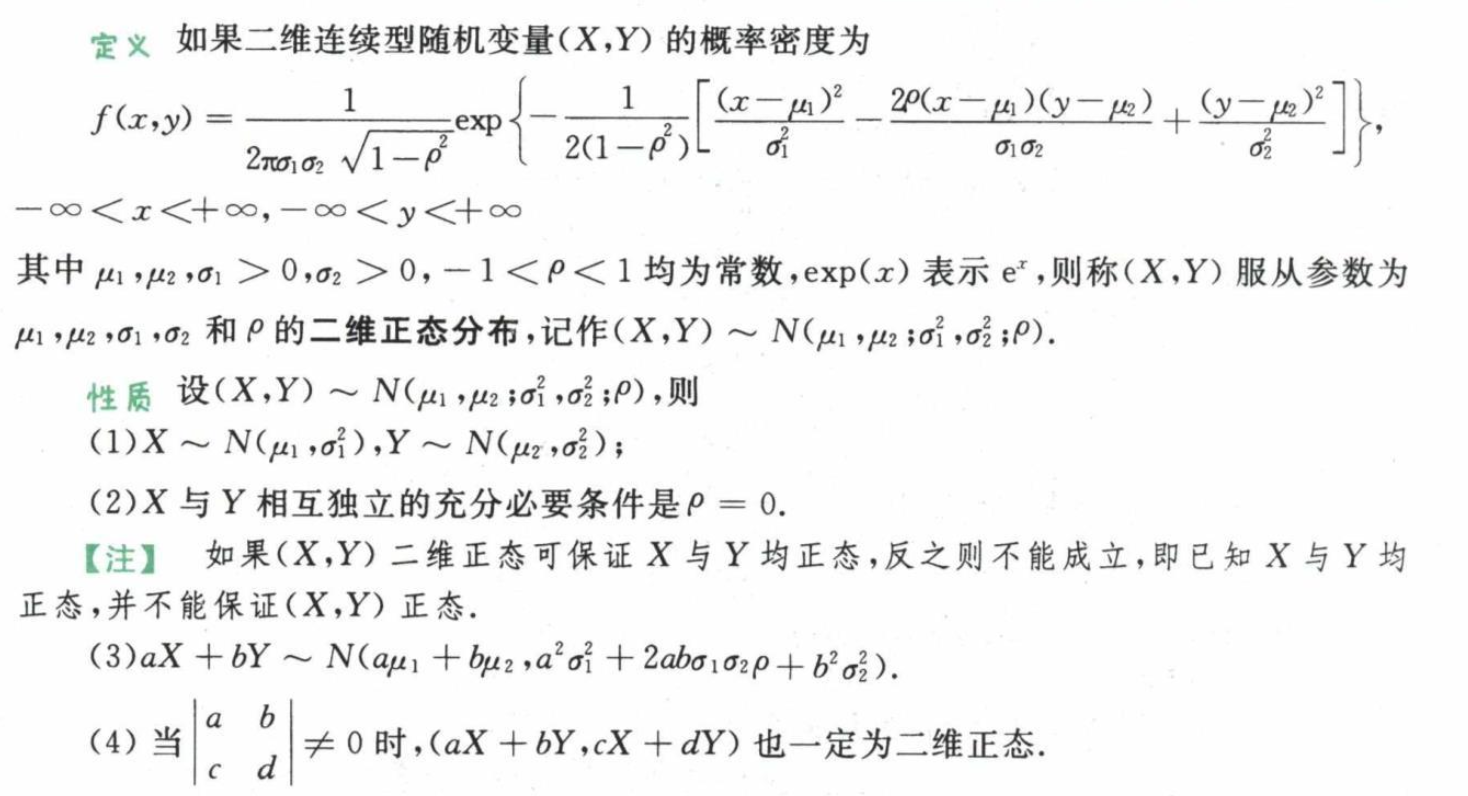
\includegraphics[width=1.2\linewidth]{pic/1.png}
      \end{center}
    \end{itemize}

\item Z = g(X, Y) 的分布
\\
主要做题方法

\end{itemize}

\textbf{随机变量的数字特征:}
\begin{itemize}
\item 随机变量的数学期望和方差

\begin{itemize}
  \item 数学期望 \(E(X)\) 是随机变量 \(X\) 的平均值,定义为:
    \begin{itemize}
      \item 离散型: \(E(X) = \sum_{i} x_i P(X = x_i)\)
      \item 连续型: \(E(X) = \int_{-\infty}^{+\infty} x f(x) dx\)
    \end{itemize}
  \item 方差 \(Var(X)\) 是随机变量 \(X\) 的离散程度,定义为:
    \begin{itemize}
      \item \(Var(X) = E[(X - E(X))^2]\)
      \item \(Var(X) = E(X^2) - [E(X)]^2\)
    \end{itemize}
  \item 协方差和相关系数:
    \begin{itemize}
      \item 协方差: \(Cov(X, Y) = E[(X - E(X))(Y - E(Y))]\)
      \item 相关系数: 
        \[
        \rho_{XY} = \frac{Cov(X, Y)}{\sqrt{Var(X) Var(Y)}}
        \]
    \end{itemize}

  \item 数学期望的性质:
    \begin{itemize}
      \item 线性性质: \(E(aX + bY) = aE(X) + bE(Y)\)
      \item 常数的期望: \(E(c) = c\)(\(c\) 为常数)
      \item 期望的加法: \(E(X + Y) = E(X) + E(Y)\)
      \item 期望的乘法: \(E(XY) = E(X)E(Y)\)(当 \(X\) 和 \(Y\) 独立时)
    \end{itemize}
  \item 方差的性质:
    \begin{itemize}
      \item \(Var(aX + b) = a^2 Var(X)\)
      \item \(Var(X + Y) = Var(X) + Var(Y) + 2Cov(X, Y)\)
      \item \(Var(X - Y) = Var(X) + Var(Y) - 2Cov(X, Y)\)
    \end{itemize}

\end{itemize}

\item 矩、协方差和相关系数

\begin{itemize}
  \item k阶原点矩:
    \[
    E(X^k) = \int_{-\infty}^{+\infty} x^k f(x) dx
    \]
  \item k阶中心矩:
    \[
    \mu_k = E[(X - E(X))^k] = \int_{-\infty}^{+\infty} (x - E(X))^k f(x) dx   
    \]
  \item k+l阶混合矩:
    \[
    E(X^k Y^l) = \int_{-\infty}^{+\infty} x^k y^l f(x, y) dx dy
    \]
  \item k+l阶混合中心矩:
    \[
    \mu_{k,l} = E[(X - E(X))^k (Y - E(Y))^l] = \int_{-\infty}^{+\infty} (x - E(X))^k (y - E(Y))^l f(x, y) dx dy
    \]
  \item 协方差:
    \[
    Cov(X, Y) = E[(X - E(X))(Y - E(Y))] = E(XY) - E(X)E(Y)
    \]
  \item 相关系数:
    \[
    \rho_{XY} = \frac{Cov(X, Y)}{\sqrt{Var(X) Var(Y)}} = \frac{E[(X - E(X))(Y - E(Y))]}{\sqrt{E[(X - E(X))^2] E[(Y - E(Y))^2]}}
    \]
  如果为独立随机变量,则相关系数为0。\\
  \(\rho_{XY} = 1\)的充分必要条件是存在常数 \(a, b\) 其中a不为0,使得
  \[
    P{Y = aX + b} = 1
  \]

  \item 协方差的性质:
    \begin{itemize}
      \item \(Cov(X, Y) = E(XY) - E(X)E(Y)\)
      \item \(D(X + Y) = D(X) + D(Y) + 2Cov(X, Y)\)
      \item \(Cov(X, Y) = Cov(Y, X)\)
      \item \(Cov(X + Y, Z) = Cov(X, Z) + Cov(Y, Z)\)
      \item \(Cov(aX + bY, Z) = aCov(X, Z) + bCov(Y, Z)\)
      \item \(Cov(X, Y) = 0\) 当且仅当 \(X\) 和 \(Y\) 独立
    \end{itemize}

\end{itemize}

\end{itemize}


\textbf{大数法则和中心极限定理:}




\textbf{数理统计}

\begin{itemize}

\item 总体、样本和统计量和样本数字特征

\item 常用统计抽样分布
\begin{itemize}
  \item \(\chi^2\) 分布: 用于检验总体方差的假设,样本方差的分布。
  \item t 分布: 用于小样本总体均值的假设检验,样本均值的分布。
  \item F 分布: 用于两个样本方差的比较,样本方差比的分布。
  \item 正态总体的抽样分布
\end{itemize}

\end{itemize}

\textbf{参数估计}
\begin{itemize}
\item 点估计

\item 估计量的求法和区间估计
\end{itemize}
\textbf{假设检验}

\end{multicols}

\end{document}